\chapter{Zeitkontrolle}

Für die Zeitkontrolle wurden die Daten aus Jira ausgewertet und im foglenden analysiert.

\section{Zeitaufwand pro Person }

\begin{figure}[H]
	\centering
	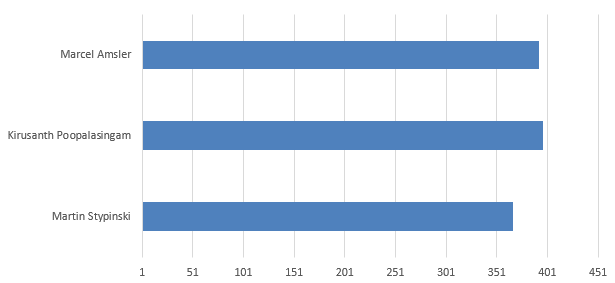
\includegraphics[width=0.8\textwidth] {images/time-per-person.png}
	\caption{Zeitaufwand pro Person in Stunden}
	\label{fig:time}
\end{figure}

Die Grafik \ref{fig:time} zeigt die total aufgewendeten Stunden pro Teammitglied.
Es wurden deutlich mehr Stunden geleistet, als die geforderten 350h gemäss ECTS.
Dies ist darauf zu begründen, dass für die Implementierung mehr Stunden als geplant aufgewendet wurden.
Denn es wurde im Team entschieden das die Applikation als Software as a Service zu entwickeln.
Um in verwendbares Ergebnis vorzeigen zu können, wurde auch eine Version für den Testzweck online gestellt.

\section{Zeitaufwand nach Task}
\begin{figure}[H]
	\centering
	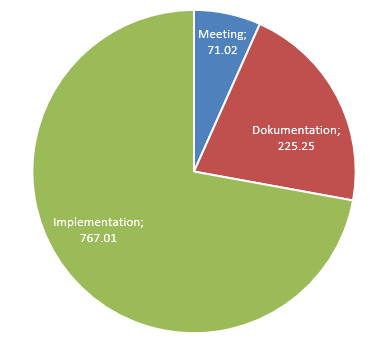
\includegraphics[width=0.4\textwidth] {images/time-per-category.png}
	\caption{Zeitaufwand pro Person in Stunden}
	\label{fig:time-per-category}
\end{figure}

Wie aus der Grafik \ref{fig:time-per-category} zu sehen ist, wurde für die Implementierung die meiste Zeit aufgewendet.
Da das Testing bei uns zur Implementierung gehört (siehe Kapitel \ref{quality-assurance} Qualitätssicherung ), ist dies nicht separat erfasst.
Zum Meeting gehören, neben dem Treffen mit dem Betreuer, und der Präsentation, auch jeweils längere interen Diskussion im Team.

